% LaTeX Article Template - customizing header and footer
\documentclass{article}

\newtheorem{thm}{Theorem}

% Set left margin - The default is 1 inch, so the following 
% command sets a 1.25-inch left margin.
\setlength{\oddsidemargin}{0.25in}

% Set width of the text - What is left will be the right margin.
% In this case, right margin is 8.5in - 1.25in - 6in = 1.25in.
\setlength{\textwidth}{6in}


% Set top margin - The default is 1 inch, so the following 
% command sets a 0.75-inch top margin.
\setlength{\topmargin}{-0.25in}

% Set height of the header
\setlength{\headheight}{0.3in}

% Set vertical distance between the header and the text
\setlength{\headsep}{0.2in}

% Set height of the text
\setlength{\textheight}{9in}

% Set vertical distance between the text and the
% bottom of footer
% Set the beginning of a LaTeX document
\usepackage{multirow}
\usepackage{fullpage}
\usepackage{graphicx}
\usepackage{amsthm}
\usepackage{amssymb}
\usepackage{algpseudocode}
\usepackage{tikz-qtree}
\usepackage{qtree}
\usepackage{amsmath}



\graphicspath{ {images/} }


\begin{document}\title{CSCI-B657 \\Assignment 3: Object detection}         % Enter your title between curly braces
	\author{Raghuveer Krishnamurthy Kanchibail\\ Supreeth Keragodu Suryaprakash \\ Suhas Jagadish \\ }        % Enter your name between curly braces
	\date{\today}          % Enter your date or \today between curly braces
	\maketitle
	
	\makeatother
	
	\pagestyle{plain}
	
	Part 1: A simple baseline
	\begin{enumerate}
		\item Subsample the images to a fixed size. Then convert each image into a vector by concatenating the rows of the image, e.g. converting a 40x40 pixel image into a 1600-dimensional vector. \newline \newline
		Solution: In order to subsample the images, we use the "extract\_feature" function defined in "NearestNeighbor.h" header. \newline
		- This function will extract the features of the input image by resizing the image to 40*40 pixel and unrolls the instance of the image on x-axis. \newline
		- Results are stored in a vector "sample" of type CImg$<$double$>$. \newline
		
		\item Call an SVM library or program to train an SVM on this task. \newline \newline
		Solution: We downloaded the SVM\_multiclass classifier from: https://www.cs.cornell.edu/people/tj/svm\_light/
		svm\_multiclass.html. We tested the classifier using the example problem provided in the website and studied the input file format. \newline
		- The vector generated above is written to a output file such that the format is compatible with the input format of SVM(Class1 Pixel1:Feature1 Pixel2:Feature2 ...). \newline
		- We use the below system() call to execute the program directly on the command line and parse the output files to the SVM classifier. \newline \newline
		system("cd SVM/ \&\& ./svm\_multiclass\_learn -c 5000 train.dat model"); \newline
		
		
		\item Then, given a new image, your testing program should apply the SVM to estimate the correct class for each test image. How well does your program work, both quantitatively and qualitatively? Does it make a difference if you use color or not? \newline
		Solution: Once the SVM model is generated, we test our program on the test images using the below system call- \newline \newline 
		system("cd SVM/ \&\& ./svm\_multiclass\_classify test.dat model prediction");\newline \newline
		- We perform the entire operation(obtaining the feature points and calling SVM classifier) for both grayscale and color images. The runtime and accuracy changes each time quantitatively and qualitatively. \newline
		- For color images, we get an accuracy of 19\% with a runtime of 20 seconds. For grayscale images, we get an accuracy of 11\% with a runtime of 10 seconds. Hence we can say that the program works well quantitatively and qualitatively for color images as compared to grayscale. \newline
		- Entire code for this implementation is stored in "Baseline.h" and we call the train and test functions using "a3.cpp". \newline
		- In order to run the grayscale algorithm, please use the algo name as "baseline\_b" and to run the color algorithm, use the algo name as "baseline\_c". \newline
		
		\begin{center}
			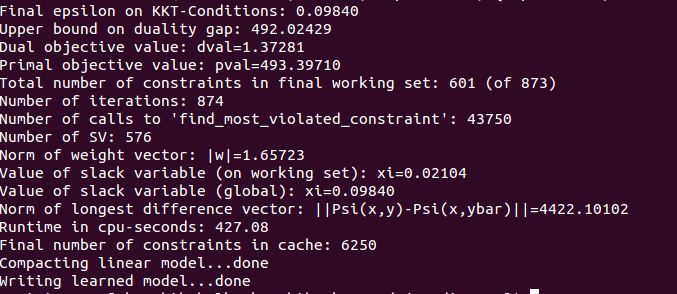
\includegraphics[width=14cm, height=4cm]{train_baseline_c.png} \\
			Figure a. Train screenshot for Baseline color
		\end{center}
		
		\begin{center}
			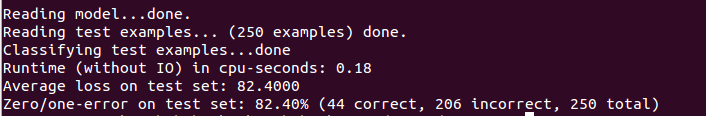
\includegraphics[width=14cm, height=2cm]{test_baseline_c.png} \\
			Figure b. Test screenshot for Baseline color
		\end{center}
		
		\begin{center}
			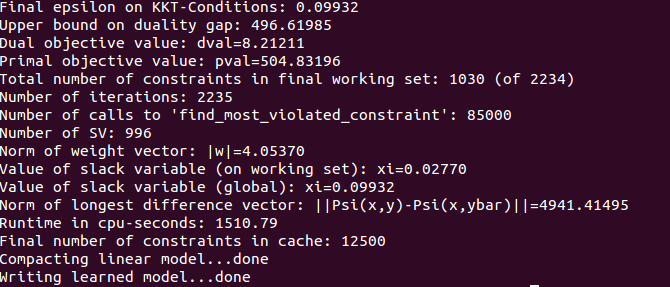
\includegraphics[width=14cm, height=4cm]{train_baseline_b.png} \\
			Figure c. Train screenshot for Baseline grayscale
		\end{center}
		
		\begin{center}
			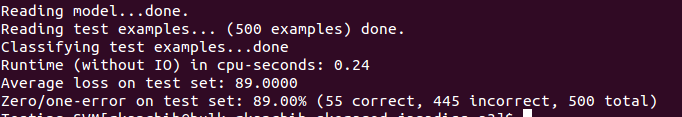
\includegraphics[width=14cm, height=2cm]{test_baseline_b.png} \\
			Figure d. Test screenshot for Baseline grayscale
		\end{center}
		
	\end{enumerate}
	
	Part 2: Traditional features
	\begin{enumerate}
		\item Eigenfood. Apply Principal Component Analysis (PCA) to the training set of grayscale feature vectors extracted above. What do the top few Eigenvectors look like, when plotted as images? How quickly do the Eigenvalues decrease? 
		Using the top k eigenvectors, represent each image as a k-dimensional feature vector by projecting the image into this lower-dimensional space. Then use an SVM similar to the one above. \newline
		Solution: We start by storing all our images into a matrix of dimension 1600*1250. 1600 since each image is reduced to 40*40 pixel image and 1250 is for total number of images. \newline
		- Next we will compute the mean matrix which contains the mean value for each row of the above generated matrix. \newline
		- After the mean is calculated, we subtract the original matrix with the mean matrix and take the transpose of the result. \newline
		- The resultant matrix will then be multiplied with the transpose of itself, giving us the covariance matrix. \newline
		- Now we use the symmetric-eigen function on the covariance matrix which gives us a matrix of eigenvectors. \newline
		- We then select top 'k' columns from the above matrix, resulting in a reduce matrix of dimensions 1250*k. \newline
		- The vector is written to a file(train.dat) which is compatible with the input format of SVM. SVM classifier is run on both train and test images and the accuracy is recorded. \newline
		- Entire code for this implementation is stored in "Eigen.h" and we call the train and test functions using "a3.cpp". \newline
		\begin{center}
			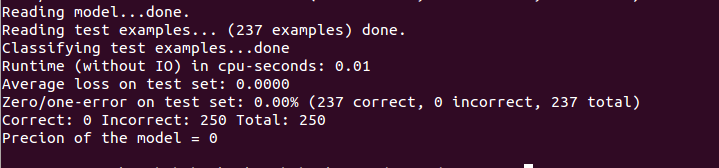
\includegraphics[width=14cm, height=2cm]{test_eigen.png} \\
			Figure a. Test screenshot for PCA
		\end{center}
		
		\item Haar-like features. Similar to Viola and Jones, define a set of many of sums and differences of rectangular regions at different positions and sizes in different configurations. Use Integral Images to compute these efficiently. Instead of Adaboost or the cascaded classifier used in Viola-Jones, simply compute each feature for each image, put them in a feature vector, and use an SVM to do the classification. \newline
		Solution: First step in generating Haar-like features is to define thousands of rectangular regions at different positions and sizes. \newline
		- We have defined a 2D vector of size 1000*4 filled with random generated values containing x, y, width and height, such that the symmetry is maintained. \newline		
		- We then resize each of the image as 40*40 pixels image. Now for each of the x and y points from the above vector, we compute the sum of all pixels(using w and h values) in this region and we call this as the white space sum. Similarly we will form a rectangle of the same size just below the white region and compute sum of all pixels to form a gray space sum. \newline 
		- We will compute the absolute difference of both the summations(white space - gray space) and pass it to a vector. The difference is computed for each image in a similar way and stored in the vector. Size of this vector is "number of images * 1000". \newline 
		- This vector is then passed to SVM classifier with the input compatible format. We train the model first and compute the accuracy for test images. \newline
		- Entire code for this implementation is stored in "haar.h" and we call the train and test functions using "a3.cpp". \newline
		- NOTE that we did last minute changes to our "haar.h" function but couldn't get time to upload the latest model. We have attached the previous model file and screenshot which gave just 1\% result. But we are sure that modified function gives us more accuracy(we have put it to run but unfortunately it is running for long). Hence please re-run "haar.h" with "train" and "test" and check the accuracy.
		\begin{center}
			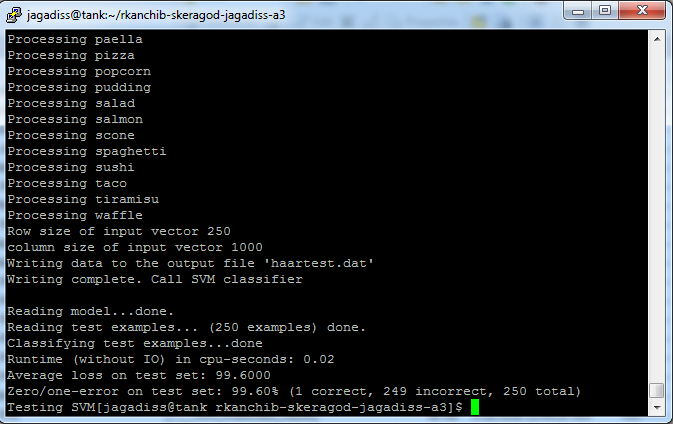
\includegraphics[width=14cm, height=2cm]{test_haar.png} \\
			Figure a. Test screenshot for haar-like features
		\end{center}
		
		\item Bags-of-words. Run SIFT on the training images, and
		then cluster the 128-d SIFT vectors into k visual words. Represent each training image as a histogram over these k words, with a k-dimenional vector. Learn an SVM similar to the one above. \newline \newline
		Solution: We start by computing SIFT descriptors for each image in the "train" directory and store the results in a vector of vectors. \newline
		- Descriptor values in Vector of vectors is copied to a Matrix object such that the Matrix holds the total number of descriptors across all images(rows) and their corresponding SIFT values(columns). We keep a reference of which image consists of which descriptors using a "ref" array. \newline
		- We then cluster the SIFT descriptor values using k-means. We have used opencv implementation of kmeans, which takes the above created Matrix as input and computes k clusters(k set to 1000 in our case). \newline
		- We will then represent each training image as a histogram over the k visual words generated above and the result is stored in "buf" vector. Essentially the vector consists of k dimensions for each image and value represents the count of SIFT descriptors for each k. \newline
		- The vector is written to a file(train.dat) which is compatible with the input format of SVM. SVM classifier is run on both train and test images and the accuracy is recorded. \newline
		- Entire code for this implementation is stored in "bow.h" and we call the train and test functions using "a3.cpp". \newline
		\begin{center}
			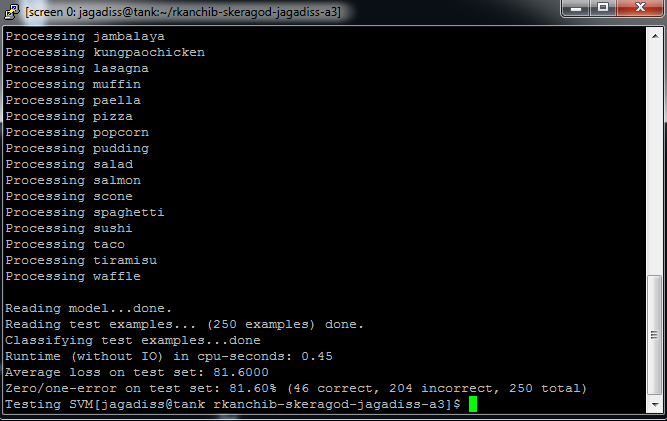
\includegraphics[width=14cm, height=2cm]{bow.png} \\
			Figure a. Test screenshot for Bag of Words
		\end{center}
	\end{enumerate}
	
	Part 3: Deep features
	\begin{enumerate}
		\item Convolutional Neural Networks for image classification. A variation on this approach is to take a pre-trained network, and instead of re-training it on a new problem, simply use the output of one of a deep but not final layer as features for input to another classifier. Your program can then input the file of
		features, and learn and test an SVM using those feature vectors. \newline \newline
		Solution: We used the OverFeat(Convolutional Network-based) feature extractor from http://cilvr.nyu.edu/doku.php?id=software:overfeat:start. In order to extract the features out of OverFeat, we use the below command- \newline \newline
		./bin/linux\_64/overfeat -f train/bagel/37105.jpg \newline \newline
		- We first convert the image to grayscale, resize it to 40*40 pixel image and then pass it to OverFeat. This optimizes the runtime of the program. \newline
		- Extracted features of each of the resized image is stored in a intermediate pipe, using which we will read the feature values(non-zero feature values as specified in the SVM classifier description) and write it to a file compatible with the input SVM format. \newline
		- Entire code for this implementation is stored in "CNN.h" and we call the train and test functions using "a3.cpp". \newline
		
		\begin{center}
			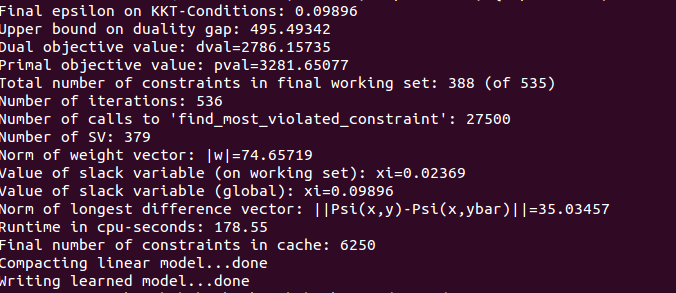
\includegraphics[width=14cm, height=4cm]{cnn_train.png} \\
			Figure a. Train screenshot for cnn
		\end{center}
		
		\begin{center}
			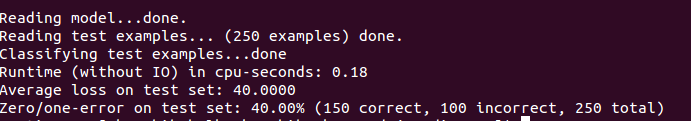
\includegraphics[width=14cm, height=2cm]{cnn_test.png} \\
			Figure b. Test screenshot for cnn
		\end{center}
		
	\end{enumerate}

Assumption:
\begin{enumerate}
	\item While running the CNN algorithm, we had to access the images in our path dynamically. Hence we have used the value of our folder name i.e., "rkanchib" as one of the inputs. Screenshot below - 
	\begin{center}
		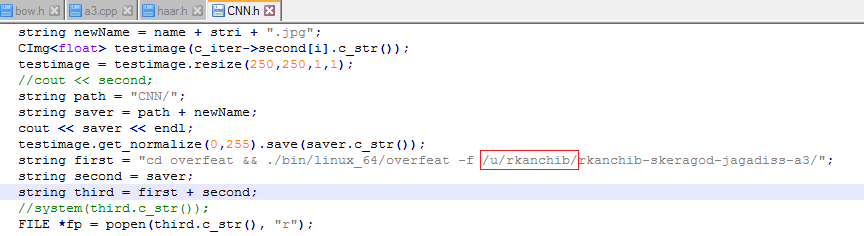
\includegraphics[width=14cm, height=4cm]{assumption.png} \\
	\end{center}
	Hence you need to modify the highlighted line in "CNN.h" to include your folder name i,e., \newline \newline
	string first = "cd overfeat \&\& ./bin/linux\_64/overfeat -f /u/"YOUR FOLDER NAME"/rkanchib-skeragod-jagadiss-a3/"; \newline \newline
	You need to make this change for 25 lines in the file "CNN.h"(for 25 classes). We regret for the trouble since we couldn't come up with a better solution in time. \newline \newline
	Also as explained in the CNN description above, we are optimizing the process by converting each image to 40*40 pixel image. Since OverFeat requires image as the parameter, we have created a separate folder called "CNN"(inside our directory) and we store all the resized images in this folder. Hence our code also demands a folder named "CNN" and in order to test CNN, the resized images should be present here. \newline
	So please run the "train" command before "test"(If you directly run the "test" against the model we gave, it will give an error since the images are not uploaded to github) \newline
	
	\item We haven't added the OverFeat package in the git directory since the file size was 1.3GB. Please install the package before executing CNN algorithm. \newline
	
	\item We have downloaded SVM classifier in a separate folder named "SVM". All the algorithms assume that SVM is installed in a folder named "SVM" and executes. You need to install SVM classifier in a separate folder named "SVM" inside our github folder in order to run the code.
	
\end{enumerate}

Experimental comparison: 
\begin{enumerate}
	\item Below table gives us an overview of the accuracies and runtimes of different algorithms. In general, we can see that CNN gives us a better accuracy with considerable runtime as compared to other algorithms.

	\begin{table}[!htbp] \centering 
		\caption{Experimental comparison} 
		\label{} 
		\begin{tabular}{@{\extracolsep{5pt}} cccc} 
			\\[-1.8ex]\hline 
			\hline \\[-1.8ex] 
			& Algorithm & Accuracy & Runtime(approx) \\ 
			\hline \\[-1.8ex] 
			1 & Baseline color & 17.6\% & 15 minutes \\ 
			2 & Baseline grayscale & 11\% & 20 minutes \\ 
			3 & PCA & 0\% & 20 minutes \\ 
			4 & Haar & 1\% & 25 minutes \\ 
			5 & BOW & 18.4\% & 30 minutes \\ 
			6 & CNN & 40\% & 20 minutes \\  
			\hline \\[-1.8ex] 
		\end{tabular} 
	\end{table}
\end{enumerate}

\end{document}